\section{Theoretische Grundlagen}
Martin F�rg hat in seiner MKS-Vorlesung sowie in seiner Dissertationsschrift
\cite{Foer06,Foer07} die theoretische Basis und den mathematischen Hintergrund f�r
\MBSim{} ausf�hrlich erkl�rt. Hier soll nur ein kurzer Einblick in die Objektorientierung
und Code-Struktur von \MBSim{} gegeben werden -- frei von der Mathematik und Mechanik, die
zur jeweiligen Beschreibung verwendet wird. Abbildung~\ref{fig:objects} zeigt hierzu
exemplarisch ein System aus Umwelt und zwei K�rpern. Angedeutet sind Wechselwirkungen
dieser untereinander �ber Kontakte und Verbindungen sowie eine �u�ere Last.

%-%-%-%-%-%-%-%-%-%-%-%-%-%-%-%-%-%-%-%-%-%-%-%-%-%-%-%-%-%-%-%-%-%-%-%-%-%-%-%-%-%-%-%-%-%-%-%
\begin{figure}[htb]
  \centering
  \psfrag{Port}[lc][lc]{\textsf{\small Port}}
  \psfrag{Body}[lc][lc]{\textsf{\small Body}}
  \psfrag{Connection}[lc][lc]{\textsf{\small Connection}}
  \psfrag{Contact}[lc][lc]{\textsf{\small Contact}}
  \psfrag{Contour}[lc][lc]{\textsf{\small Contour}}
  \psfrag{Load}[lc][lc]{\textsf{\small Load}}
  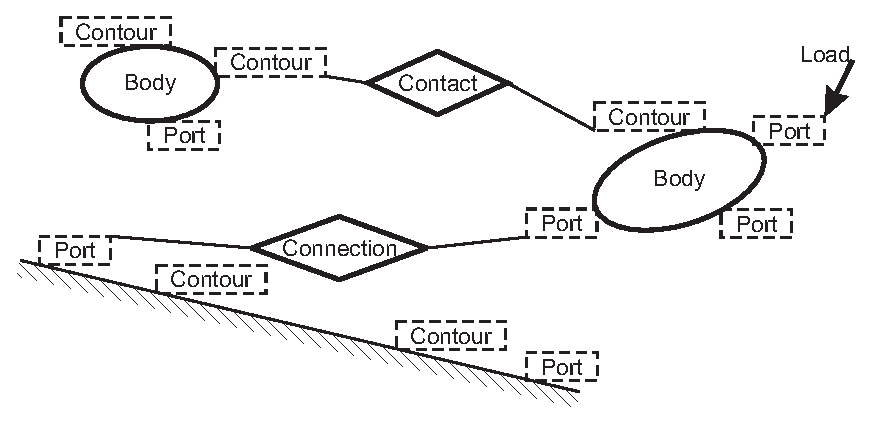
\includegraphics[width=0.8\hsize]{objectorientationMBSim.eps}
  \caption{Objekt-Strukturierung in \MBSim{}}
  \label{fig:objects}
\end{figure}
%-%-%-%-%-%-%-%-%-%-%-%-%-%-%-%-%-%-%-%-%-%-%-%-%-%-%-%-%-%-%-%-%-%-%-%-%-%-%-%-%-%-%-%-%-%-%-%

Ein K�rper~(\texttt{Body...}) ist in \MBSim{} durch seine Lagen~$\vq$ und
Geschwindigkeiten~$\vu$ parametrisiert. Die Parameter der beschreibenden
Differentialgleichung sind bei starren K�rpern~(\texttt{BodyRigid...}) immer Masse~$m$ und
Tragheitstensor~$\vTheta$. Die Modelle f�r flexible K�rper~(\texttt{Bodyflexible...}) sind in der
Parametrisierung jeweils sehr speziell -- f�r sie sei auf die jeweiligen Implementierungen
und die zugeh�rigen Dokumentationen verwiesen.

Die Umwelt kann wie auch alle K�rper Konturen~(\texttt{Contour}) sowie
Anschl�sse~(\texttt{Port}) aufnehmen, auf denen Kontakte sowie diskrete Wechselwirkungen
definiert werden k�nnen. Zudem ist Gravitation �ber die Umwelt definiert.

Kontakte zwischen den Konturen unterschiedlicher K�rper k�nnen sowohl als
Starrk�rperkontakt~(\texttt{ContactRigid}, mengenwertig, nicht-glatte Dynamik) als auch
als nachgiebiger Kontakt~(\texttt{ContactFlexible}, funktional, lokale Steifigkeit)
definiert werden. Reibung wird hierbei jeweils durch die Angabe der auszuwertenden
Reibrichtungen eingebunden. Verbindungen zwischen zwei Anschl�ssen k�nnen sowohl starr
(\texttt{ConnectionRigid}) als auch mit Nachgiebigkeit~(\texttt{ConnectionFlexible})
modelliert werden. F�r �ussere Lasten~(\texttt{Load}) k�nnen beliebige Vorschriften
angegeben werden.

